\chapter{Methodology}

We have shown that reservoir computing using Random Boolean Networks is a feasible approach to solving binary time-series problems.
We now wish to investigate which parameters and characteristics of the reservoir lead to optimal performance and resource usage.

The following questions arise:

\begin{enumerate}
    \item How small can a RBN Reservoir System be while still solving a given task at close to 100\% accuracy?
    \item How many connections from the input layer are required to sufficiently perturb the reservoir?
    \item How few reservoir nodes can be connected to the readout layer while maintaining task accuracy?
    \item Is there a correlation between the dynamical characteristics of the RBN (number of attractors, attractor length) and its performance as a reservoir?
\end{enumerate}

The answers to these questions aren't 'just' of theoretical interest,
they also give us insight to how physical reservoir computing devices have to be instrumented.

In a physical substrate it might be prohibitively expensive or technologically infeasible to read the state of the entire reservoir,
and the nodes you are able to measure might be affected by the 'values' of the nodes next to it.
In the case of a growing and modifying reservoir, such as a stem-cell based reservoir,
the topology of the network might change over time without having the ability to reinstrument the device.
A finding that it's enough to use a subset of the available nodes for regression in the readout layer,
regardless of reservoir size, would be of practical interest.

There are two factors affecting optimal reservoir perturbance:
There might be a problem-specific optimal perturbance dependent on the task at hand as well as connectivity of the reservoir and number of runs after each perturbance.
For physical devices one is in addition limited by the physical characteristics of the reservoir,
such as cost and the number of available electrodes for instrumenting limited by physical space.

Finding the minimum required size of a RBN Reservoir for a given task allows us to create physical reservoirs with adequate computational abilities guided by the theoretical foundations described herein ("Helmax setning, Egon! Helmax!").

Finally, we attempt to explain the performance of RBN Reservoirs through their dynamical properties,
calculating the number of attractors and their length for reservoirs against their accuracy on a given task.
A correlation between these properties might be interesting, and help to explain why some reservoirs perform better than others.

\section{Experimental setup}

The final RRC system is shown as a block diagram in Figure \ref{figure:rrc-block},
and the actual network topology is equivalent to the one in Figure \ref{figure:rbn-reservoir}.

\todo{gotta add moar stuffz here, nemlig varierende input/output cocnnectivitet støtte}

\begin{figure}
  \centering
  \begin{tikzpicture}
    \node (dataset) {Dataset};
    \node[box, below=of dataset] (input) {Input layer};
    \node[box, right=of input] (reservoir) {RBN Reservoir};
    \node[box, right=of reservoir] (readout) {Readout layer};
    \node[above=of readout] (classification) {Classification};

    \node[draw,dotted,fit=(input) (reservoir) (readout), label={RRC}] {};

    \draw[edge] (dataset) to (input);
    \draw[edge] (input) to (reservoir);
    \draw[edge] (reservoir) to (readout);
    \draw[edge] (readout) to (classification);
  \end{tikzpicture}
  \caption{Block diagram of the RRC processing a dataset.}
  \label{figure:rrc-block}
\end{figure}

\subsection{testing}

To verify that RBN simulation is working,
a RBN is created randomly, initial state set to all zeros, and ran.
The results are visualized in Figure \ref{figure:rbn-noperturb}.
We see that the RBN exhibits stable dynamics, and enters into an attractor around $t=15$.
In Figure \ref{figure:rbn-perturb} we continiously perturb the RBN with the input stream from the Temporal Parity task visualized in Figure \ref{figure:temporal-parity}.
In the perturbed case, the state trajectory is continiously changed, preventing the RBN from settling into an attractor.
Interestingly enough, there seems to be a visual similarity between the two cases.
Such a pattern is sure to dissapear with a RBN in the chaotic phase.

This erratic pattern of state transitions is then fed into the readout layer,
which is then tasked with finding a linear combination of the RBN states that results in the expected output for the given task.

\begin{figure}
  \subfloat[Unperturbed]{
    
\includegraphics[width=0.5\columnwidth]{method/final-1-noperturb.pdf}
    \label{figure:rbn-noperturb}
  }
  \subfloat[Perturbed]{
    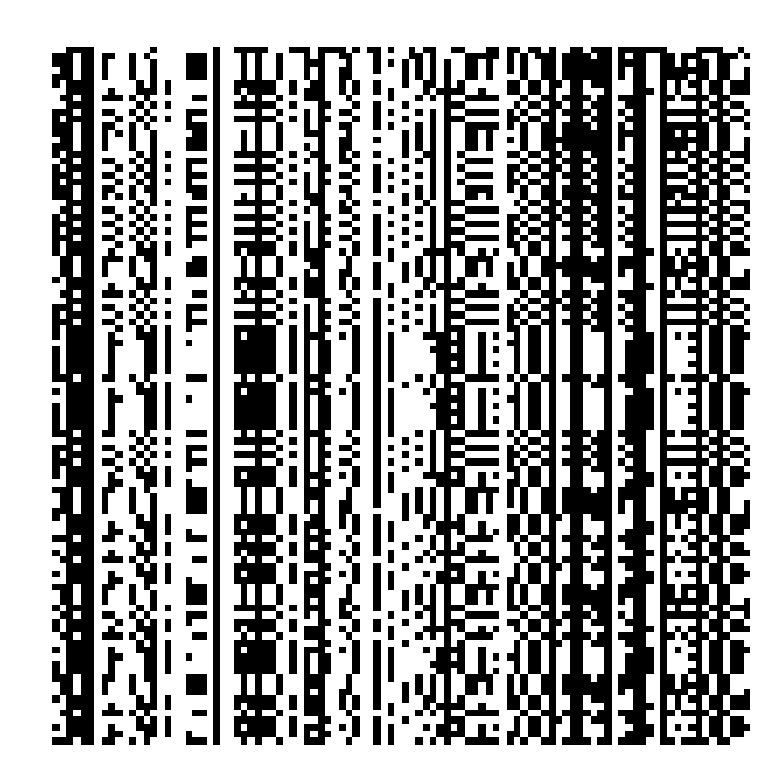
\includegraphics[width=0.5\columnwidth]{method/final-1-perturb.pdf}
    \label{figure:rbn-perturb}
  }
  \caption{
    The same RBN ($N=100, K=2, P=0.5, L=50$) shown both perturbed and unperturbed.
    The boolean states of the RBN are plotted along the X-axis,
    with time flowing downwards.
  }
\end{figure}

\subsection{Training}

To train the RRC system we require large training datasets,
as well as different, smaller datasets for testing the trained system.
We will use the datasets described in section \ref{subsection:rbn-reservoir-systems}.

We then either create a new RBN (initialize it randomly),
or load a previously created RBN from disk.
For each bit of input in each dataset,
we perturb the input-connected nodes in the RBN.
After each perturbance, the RBN is ran synchronously (CRBN mode) for one timestep.
The resulting RBN states are collected,
and after the entire dataset is processed,
forwarded to the readout layer.

To find a suitable mapping from the set of reservoir states and the correct input classification,
ridge regression \cite{hoerl1970ridge} is used.
This version of least squares regression is more accurate when faced with input colinearities, as well as always being at least as accurate as ordinary least squares.  
This process is repeated for all the datasets,
and the final regression parameters are chosen as a combination of the parameters obtained for each individual dataset.
Finally we measure the normalized accuracy of the trained reservoir on the test dataset,
defined as the following:
\begin{equation}
Accuracy = 1 - \dfrac{sum(actual\_output \neq expected\_output)}{len(correct\_output)}
\label{formula:accuracy}
\end{equation}

\section{Finding the minimum required reservoir size, optimal input connectivity}

As shown in my previous paper \cite{MyPreviousPaper},
there are a plethora of RRC systems with $N=100, K=\{2, 3\}$ that solve the Temporal Parity task for a window size of both 3 and 5,
The reservoirs with $K=3$ had a higher density of success in general,
and the larger reservoirs fared better on the task with window size 5.

Presumably the same tasks can be solved with smaller reservoirs,
the question being how small they can be while retaining accurarcy.
As the optimal reservoir size and input connectivity might depend on the task at hand,
we test our reservoirs on both the Temporal Parity \ref{missing} and Temporal Density \ref{missing}
tasks with window sizes of both 3 and 5 (as specified in table \ref{tab:tasks}).

\begin{table}[ht]
  \centering
  \caption{Task parameters}
  \label{tab:tasks}
  \begin{tabular}{ll}
    Task type               & Temporal Parity and Density \\
    Training dataset length & 4 000                       \\
    Test dataset length     & 200                         \\
    $N$ (window size)       & 3 and 5                     \\
    $t$ (offset)            & 0
  \end{tabular}
\end{table}

To find the optimal reservoir size and input connectivity,
we'll randomly initialize 50 reservoirs for each combination of the reservoir parameters in table \ref{tab:ic-reservoir-parameters}.

For our experiments we'll only be looking at reservoirs with $K=3$.
As well as being more useful due to the homogenous degree of the network (to simulate $\langle K \rangle = 2 $) and
having a higher population accuracy, it reduces the number of parameter combination we have to simulate.

\begin{table}[ht]
    \centering
    \caption{Reservoir parameters for optimal input connectivity}
    \label{tab:ic-reservoir-parameters}
    \begin{tabular}{ll}
        Nodes               & [10..50], step size=5         \\
        Connectivity        & 3                             \\
        Input connectivity  & [0..n\_nodes], step size = 5  \\
		Output connectivity & n\_nodes                      \\
        Sample size         & 50
    \end{tabular}
\end{table}

After plotting the resulting accuracies on the previously mentioned tasks,
one should be able to visually identify the minimum required reservoir size for the given task,
as well as what the optimal input connectivity might be, as a function of reservoir size and task.

\section{Minimum required output connectivity}

How few connections can one have from the reservoir itself to the readout layer,
while staying accurate on the task at hand?
As the reservoir prediction is computed by regressing the states of the network nodes against the expected output bits,
reducing the number of nodes used in the regression can never give a higher accuracy than using all of the nodes.
If there is redundant information in the network, quite a few nodes could be cut off from the readout layer while maintaining the best accuracy for this specific reservoir.
This does require a sufficient amount of linear independence between the remaining nodes of the network.

As shown in the previous section, different problems require different reservoir sizes.
Past a certain reservoir size, all reservoirs have a sufficient accuracy on the given task.
One could postulate that for reservoirs larger than the 95\% accuracy breakpoint,
it suffices to read out a number of nodes equal to the breakpoint.
If this is the case, one can safely use growing reservoirs without having to change the output connections,
given that the reservoir was able to solve the given task in the first place.

The results from the previous section show a correlation between input connectivity and accuracy,
with the reservoirs having a input connectivity of $n\_nodes / 2$ having the highest population accuracy.
Using this information, we can reduce our search space for minimum required output connectivity considerably.
The parameters in table \ref{tab:oc-reservoir-parameters} will be used for simulation.

\begin{table}[ht]
    \centering
    \caption{Reservoir parameters for optimal output connectivity}
    \label{tab:oc-reservoir-parameters}
    \begin{tabular}{ll}
        Nodes               & [10..100], step size=10           \\
        Connectivity        & 3                                 \\
        Input connectivity  & $ n\_nodes / 2 $                  \\
        Output connectivity & [0..n\_nodes], step size=10       \\
        Sample size         & 50
    \end{tabular}
\end{table}

\section{Analyzing reservoir dynamics}
